\documentclass[border=10pt]{standalone}
% Shared style for the EMONI diagrams. Build: tectonic <file>.tex, then pdftocairo -svg.
\usepackage{fontspec}
\setmainfont{FiraSans}[Extension=.otf,UprightFont=*-Regular,BoldFont=*-SemiBold,ItalicFont=*-Italic,BoldItalicFont=*-SemiBoldItalic]
\setmonofont{FiraMono}[Extension=.otf,UprightFont=*-Regular,BoldFont=*-Medium,Scale=0.9]
\usepackage{tikz}
\usetikzlibrary{arrows.meta,positioning,shapes.geometric,shapes.misc,calc,fit,backgrounds}
\definecolor{eg}{HTML}{11903B}   % EMONI green
\definecolor{egl}{HTML}{E8F7EE}
\definecolor{eb}{HTML}{2A78D6}   % blue
\definecolor{ebl}{HTML}{EAF2FC}
\definecolor{eo}{HTML}{D9631E}   % orange
\definecolor{eol}{HTML}{FDF0E7}
\definecolor{ep}{HTML}{7C4DCC}   % purple
\definecolor{epl}{HTML}{F2ECFB}
\definecolor{er}{HTML}{C5221F}   % red
\definecolor{erl}{HTML}{FCEAEA}
\definecolor{ink}{HTML}{1F2328}
\definecolor{mute}{HTML}{59636E}
\definecolor{line}{HTML}{D0D7DE}
\tikzset{
  every node/.style={text=ink,font=\small},
  >={Stealth[length=2.4mm]},
  % sequence diagrams
  life/.style={draw=line,dashed,thick},
  head/.style={draw=#1,fill=#1!8,rounded corners=3pt,minimum width=27mm,minimum height=11mm,align=center,font=\small\bfseries,thick},
  act/.style={draw=#1,fill=#1!18,minimum width=2.2mm},
  msg/.style={->,thick,draw=ink},
  ret/.style={->,dashed,draw=mute},
  mlabel/.style={font=\footnotesize,fill=white,inner sep=1.5pt,align=center},
  note/.style={draw=#1,fill=#1!8,rounded corners=2pt,font=\footnotesize,align=left,inner sep=4pt},
  frag/.style={draw=mute,rounded corners=2pt},
  fraglabel/.style={draw=mute,fill=white,font=\footnotesize\bfseries,inner sep=2.5pt,anchor=north west},
  % activity diagrams
  start/.style={circle,fill=ink,minimum size=4mm,inner sep=0},
  stop/.style={circle,draw=ink,thick,minimum size=5mm,inner sep=0,path picture={\fill[ink] (path picture bounding box.center) circle (1.4mm);}},
  step/.style={draw=#1,fill=#1!8,rounded corners=5pt,thick,minimum height=9mm,minimum width=40mm,align=center,font=\small},
  step/.default=eg,
  dec/.style={diamond,aspect=2.2,draw=ink,fill=white,thick,inner sep=1.5pt,align=center,font=\footnotesize},
  flow/.style={->,thick,draw=ink},
  guard/.style={font=\footnotesize\itshape,text=mute,fill=white,inner sep=1.5pt},
  lane/.style={draw=line,fill=#1,rounded corners=4pt},
  lanetitle/.style={font=\small\bfseries,text=mute},
}

% Activity: one wake-up of the device, as published in the EMONI Technical Reference Manual (1.3, 2.3).
\begin{document}
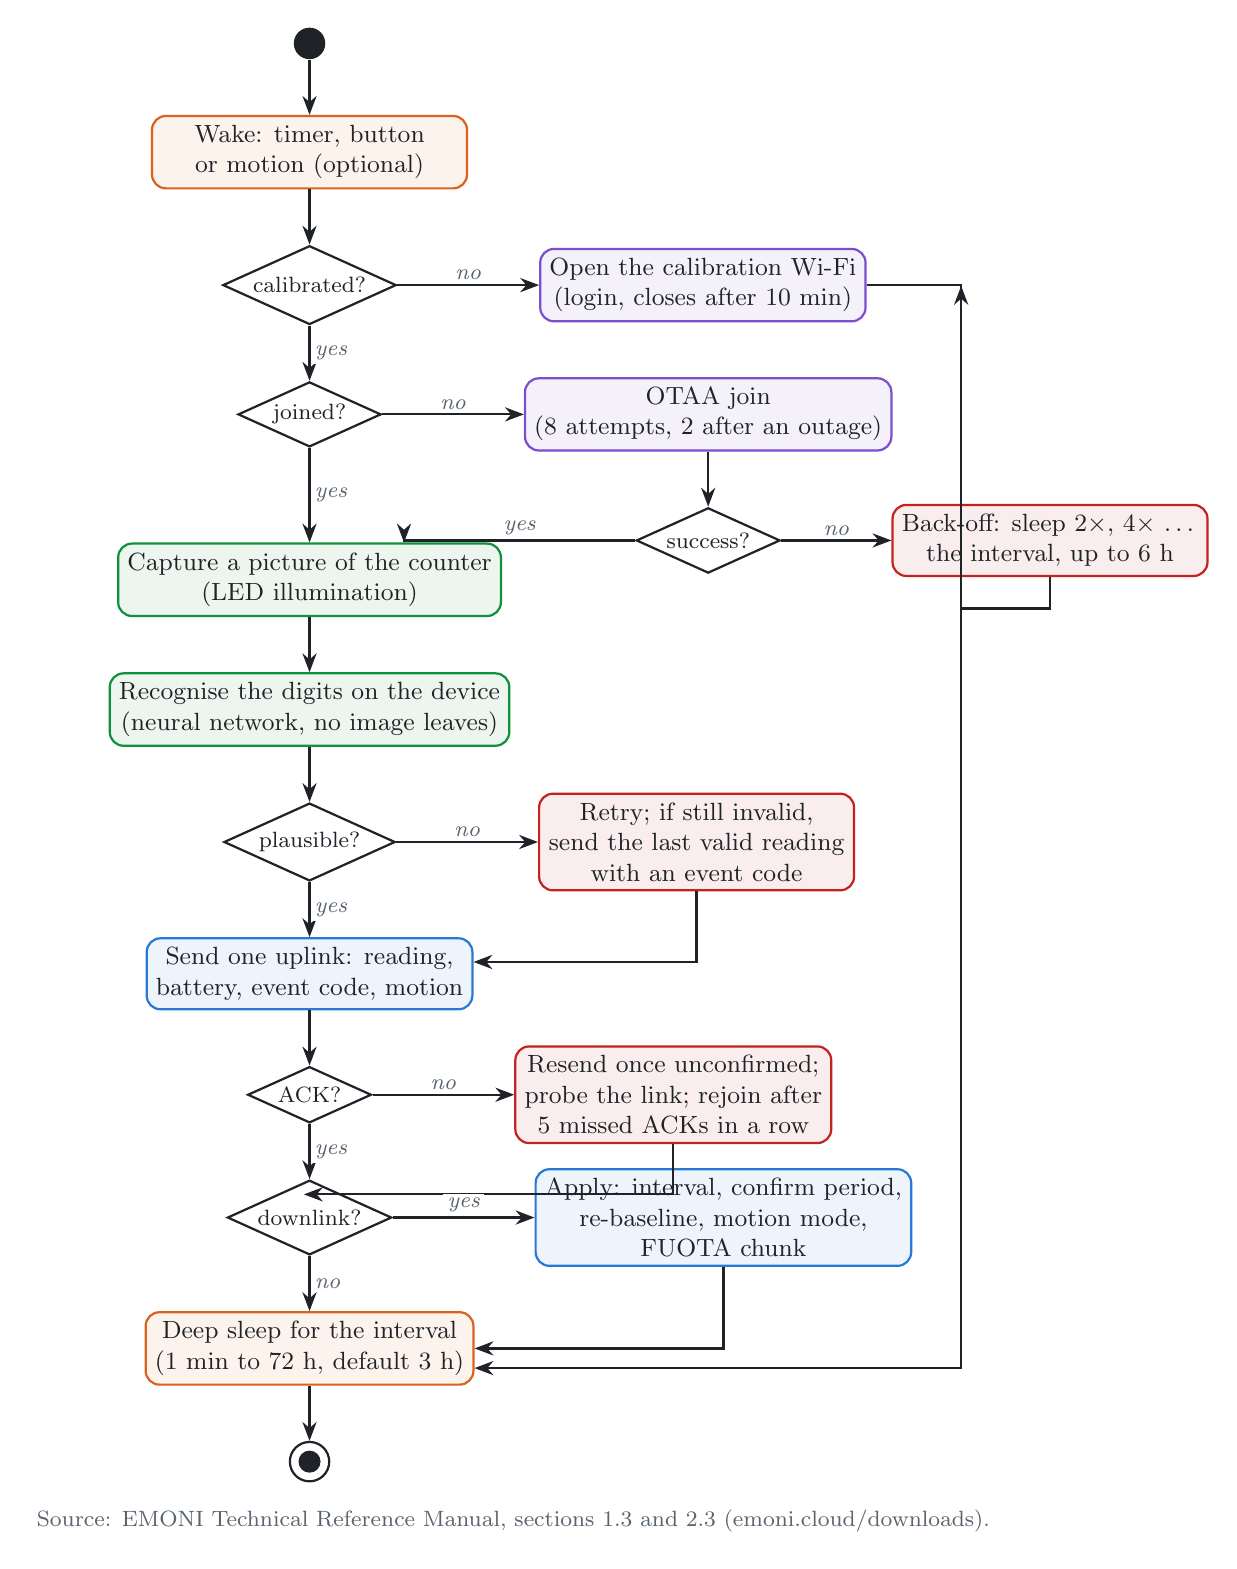
\begin{tikzpicture}[node distance=7mm and 12mm]
\node[start] (s) {};
\node[step=eo,below=of s] (wake) {Wake: timer, button\\or motion (optional)};
\node[dec,below=of wake] (cal) {calibrated?};
\node[step=ep,right=18mm of cal] (wifi) {Open the calibration Wi-Fi\\(login, closes after 10 min)};
\node[dec,below=of cal] (join) {joined?};
\node[step=ep,right=18mm of join] (dojoin) {OTAA join\\(8 attempts, 2 after an outage)};
\node[dec,below=of dojoin] (jok) {success?};
\node[step=er,right=14mm of jok] (back) {Back-off: sleep 2$\times$, 4$\times$ \ldots\\the interval, up to 6 h};
\node[step,below=12mm of join] (pic) {Capture a picture of the counter\\(LED illumination)};
\node[step,below=of pic] (ocr) {Recognise the digits on the device\\(neural network, no image leaves)};
\node[dec,below=of ocr] (ok) {plausible?};
\node[step=er,right=18mm of ok] (retry) {Retry; if still invalid,\\send the last valid reading\\with an event code};
\node[step=eb,below=of ok] (up) {Send one uplink: reading,\\battery, event code, motion};
\node[dec,below=of up] (ack) {ACK?};
\node[step=er,right=18mm of ack] (nack) {Resend once unconfirmed;\\probe the link; rejoin after\\5 missed ACKs in a row};
\node[dec,below=of ack] (dl) {downlink?};
\node[step=eb,right=18mm of dl] (apply) {Apply: interval, confirm period,\\re-baseline, motion mode,\\FUOTA chunk};
\node[step=eo,below=of dl] (sleep) {Deep sleep for the interval\\(1 min to 72 h, default 3 h)};
\node[stop,below=of sleep] (e) {};
\draw[flow] (s) -- (wake); \draw[flow] (wake) -- (cal);
\draw[flow] (cal) -- node[guard,above]{no} (wifi);
\draw[flow] (cal) -- node[guard,right]{yes} (join);
\draw[flow] (join) -- node[guard,above]{no} (dojoin);
\draw[flow] (dojoin) -- (jok);
\draw[flow] (jok) -- node[guard,above]{no} (back);
\draw[flow] (jok.west) -| node[guard,above,pos=0.25]{yes} ($(pic.north)+(1.2,0)$);
\draw[flow] (join) -- node[guard,right]{yes} (pic);
\draw[flow] (pic) -- (ocr); \draw[flow] (ocr) -- (ok);
\draw[flow] (ok) -- node[guard,above]{no} (retry);
\draw[flow] (ok) -- node[guard,right]{yes} (up);
\draw[flow] (retry.south) |- ($(up.east)+(0,0.15)$);
\draw[flow] (up) -- (ack);
\draw[flow] (ack) -- node[guard,above]{no} (nack);
\draw[flow] (ack) -- node[guard,right]{yes} (dl);
\draw[flow] (nack.south) |- ($(dl.north east)+(-0.6,0.05)$);
\draw[flow] (dl) -- node[guard,above]{yes} (apply);
\draw[flow] (dl) -- node[guard,right]{no} (sleep);
\draw[flow] (apply.south) |- (sleep.east);
\draw[flow] (wifi.east) -- ++(1.2,0) |- ($(sleep.east)+(0,-0.25)$);
\draw[flow] (back.south) -- ++(0,-0.4) -| ($(wifi.east)+(1.2,-0.01)$);
\draw[flow] (sleep) -- (e);
\node[font=\footnotesize,text=mute,anchor=north west,align=left] at ($(e.south west)+(-3.4,-0.3)$) {Source: EMONI Technical Reference Manual, sections 1.3 and 2.3 (emoni.cloud/downloads).};
\end{tikzpicture}
\end{document}
